% !TEX encoding   = UTF8
% !TEX spellcheck = ru_RU
% !TEX root = ../seminars.tex

%%================================
\section{Правильный шестиугольник}
%%================================
Рассмотрим класс \code{Regular\_hexagon} из~упражнения~8 \textbookref{главы~13}. Правильный шестиугольник, по~сути, является многоугольником \code{Polygon}. Однако он не~может содержать количество вершин, отличное от~6-ти. Таким образом, заманчиво наследовать от~\code{Polygon}, но тогда функцию \code{add()}, добавляющую дополнительные точки, необходимо как-то исключить из~интерфейса. И хотя, в~принципе, некоторые языки (с~динамической типизацией) позволяют сделать это, наследование интерфейса нарушилось бы. То есть там, где требуется \code{Polygon} мы не~смогли бы использовать \code{Regular\_hexagon}, в~который нельзя добавлять точки.

Хоть это лишает нас возможности воспользоваться реализацией классов \code{Polygon} или \code{Closed\_polyline}, \emph{логически правильным} решением является наследовать от~абстрактной фигуры \code{Shape}:

\cppfile[firstline=53, lastline=65]{projects/lib/Graph_lib/ext/graph.h}

В~конструкторе добавляем точки, используя вращательную симметрию:

\cppfile[firstline=93, lastline=107]{projects/lib/Graph_lib/ext/graph.cpp}

\noindent Округление при~помощи функции \code{std::round()} вместо отбрасывания дробной части даёт возможность слегка улучшить качество рисования в~отдельных случаях.

В~реализации следующих методов, которые предоставляются для~удобства пользователей, применяется априорное знание об~ориентации шестиугольника на~плоскости:

\cppfile[firstline=109, lastline=118]{projects/lib/Graph_lib/ext/graph.cpp}

Заметим, что эти функции можно было бы вынести из~класса, то есть сделать внешними по~отношению к~классу. Тем не~менее, мы расположили их внутри, поскольку это свойства самих объектов и эти свойства есть у~подобных объектов других типов. Например, у~окна также есть длина (\code{x\_max()}) и ширина (\code{y\_max()}).

Код оставшейся функции \code{draw\_lines()} в~точности повторяет реализацию из~классов \code{Open\_polyline} и \code{Closed\_polyline}:

\cppfile[firstline=120, lastline=142]{projects/lib/Graph_lib/ext/graph.cpp}

Пример рисования правильных шестиугольников показан на~рисунке~\ref{fig:regularhexagon}.



%%==================================
\section{Мозаика из~шестиугольников}
%%==================================
Применим разработанный класс \code{Regular\_hexagon} для~рисования мозаики в~пределах прямоугольной области из~упражнения~9 \textbookref{главы~13}.

\begin{figure}[ht]
    {\centering
        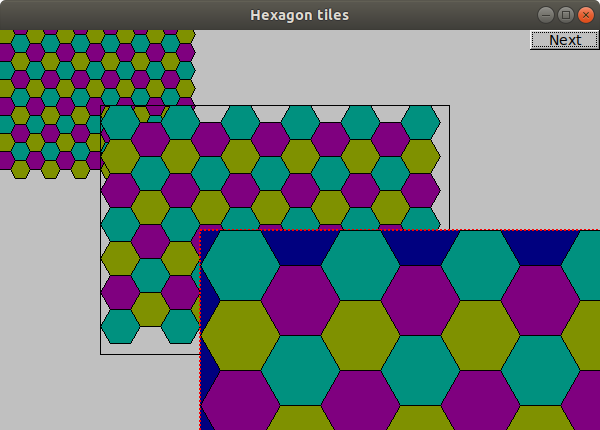
\includegraphics[width=0.6\textwidth]{images/hexagon_tiles.png}

    }
    \caption{Элементы мозаики из~правильных шестиугольников}
    \label{fig:regularhexagon}
\end{figure}

Наследование выполним от~класса \code{Rectangle}, а для~хранения множества правильных шестиугольников воспользуемся классом \code{Vector\_ref}:

\cppfile[firstline=68, lastline=79]{projects/lib/Graph_lib/ext/graph.h}

Вся работа по~формированию мозаики выполняется в~конструкторе. Параметры~\code{p}, \code{ww} и~\code{hh} задают прямоугольник, который заполняется одинаковыми правильными шестиугольниками. Размер шестиугольников определяется радиусом описанной окружности \code{rr}. Код конструктора приведён ниже:

\cppfile[firstline=144, lastline=171]{projects/lib/Graph_lib/ext/graph.cpp}

Реализация перекрывающих методов выполняется тривиально:

\cppfile[firstline=173, lastline=185]{projects/lib/Graph_lib/ext/graph.cpp}

Вначале мы рисуем прямоугольник, затем мозаику. По~умолчанию, прямоугольник не~рисуется. Это поведение мы установили в~конструкторе класса, задав невидимый цвет. Если изменить цвет рисования, то мы увидим границу (и заливку) прямоугольной области, как показано на~рисунке~\ref{fig:regularhexagon}.

\begin{figure}[ht]
    {\centering
        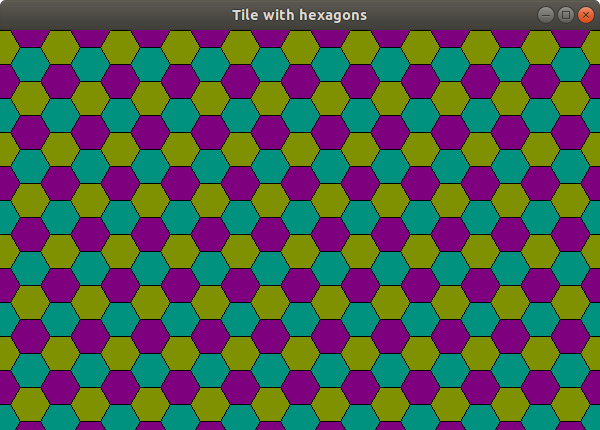
\includegraphics[width=0.6\textwidth]{images/tile_window.png}

    }
    \caption{Окно, полностью заполненное мозаикой}
    \label{fig:hexagontile}
\end{figure}

На~рисунке~\ref{fig:hexagontile} мозаикой покрыта вся область окна.
